\documentclass{article}
\usepackage{iclr2025_conference,times}
\usepackage[T1]{fontenc}
\usepackage{booktabs,tabularx,array,graphicx,placeins}
\usepackage{hyperref}
\urlstyle{same}
\iclrfinalcopy
\title{Designing an Agent Harness for\\Machine Learning Development}
\author{Weiwei Wu\\Stanford University\\\texttt{wwwu@stanford.edu}}
\hypersetup{hidelinks,pdftitle={Designing an Agent Harness for Machine Learning Development},pdfauthor={Weiwei Wu}}
\newcommand{\coderepo}{\url{https://github.com/weiweiwu007/cs329z-ml-agent}}
\begin{document}
\maketitle
\lhead{CS329Z Engineering AI Agents --- Midway Report}

\section{Research Questions or Problem Specification}
ML engineers repeatedly inspect results, choose model changes, and run experiments. We are building one agentic system to carry out this loop across MLPs, CNNs, and transformers. Given a dataset, starting model, and compute budget, it proposes changes and tests them. Our current question is: \textbf{Do detailed error reports and a separate reviewer help an agent produce better models within the same compute budget?} Following the proposal feedback, we compare four fixed harness designs to study how agents use evidence and coordinate decisions. Improving the workflow itself remains a later step.

\section{Environment \& Data}
\textbf{Tasks.} One planner and runner use task-specific data loaders, builders, and graders (Table~\ref{tab:tasks}). Our completed evaluation uses UCI Covertype \citep{blackard1998covertype}. Its 581,012 labeled land cells have 54 terrain and soil features and seven forest cover classes, derived from US Forest Service and US Geological Survey records. Covertype replaced a Spambase pilot that left little room for improvement.

\begin{table}[h]
\caption{Three model families. Only the Covertype study has completed the current evaluation.}
\label{tab:tasks}
\centering
\begin{tabularx}{\linewidth}{@{}>{\raggedright\arraybackslash}p{0.68in}>{\raggedright\arraybackslash}X >{\raggedright\arraybackslash}p{1.30in}>{\raggedright\arraybackslash}p{0.91in}@{}}
\toprule
\textbf{Model} & \textbf{Task and dataset} & \textbf{Starting model} & \textbf{Score; status}\\
\midrule
MLP & Forest cover classification; Covertype & Two hidden layers: 128, 64 units; from scratch & Accuracy; completed\\
CNN & 100-class image classification; CIFAR-100 & CIFAR ResNet-18; from scratch & Top-1 accuracy; runs pending\\
Transformer & Sentiment: SST-2; paraphrases: MRPC & Pretrained BERT-Tiny with a fresh classifier & Accuracy; MRPC F1; runs pending\\
\bottomrule
\end{tabularx}
\end{table}

\textbf{Evaluation data.} We construct a stratified 60/20/20 train/validation/test split of Covertype with split seed 20261104. Preprocessing statistics are fitted on training data only. The downloaded archive hash and split indices are recorded. Agents see training and validation results. A separate evaluator scores the selected model on test labels hidden from the agents. The planned image and text tasks use CIFAR-100 and GLUE \citep{krizhevsky2009cifar,wang2019glue}; their evaluation runs are pending.

\textbf{Resources and allowed changes.} The Covertype baseline is a $54\!\rightarrow\!128\!\rightarrow\!64\!\rightarrow\!7$ MLP trained for five epochs with AdamW, learning rate 0.001, batch size 128, cosine decay, and dropout 0.1. Agents can change layer sizes, training length, optimizer settings, batch size, schedules, regularization, normalization, and supported preprocessing. Numeric settings are free within constraints, including a 500,000-parameter cap. Each run allows at most 20 attempts and 80 API calls. We evaluated 168-second and 600-second budgets with three matched seeds per design, one NVIDIA L4 per run, and the same \texttt{openai/gpt-6-luna} API model.

\textbf{Success criteria.} We measure best validation accuracy against cumulative compute, then test the selected model. We also record attempts, model size, timeouts, API cost, and agent decisions. Charged compute includes the baseline, worker execution, and diagnostics; API waiting and process startup are recorded separately. Thus equal compute does not mean equal total cost. All scores are calculated by code, not by an LLM judge.

\section{Methods}
\textbf{The harness.} As in Homework 1, the harness controls context, tool execution, and stopping. DSPy handles structured model calls \citep{khattab2023dspy}; Pydantic checks the returned fields; LangGraph connects the stages and checkpoints workflow state \citep{langchain2026langgraph}. Trusted Python code builds, trains, and scores each proposed model.

\begin{enumerate}
\item \textbf{Plan.} Given the task, previous results, and remaining budget, the planner returns an observation, hypothesis, predicted effect, experiment, full model recipe, and supporting trial IDs.
\item \textbf{Validate and execute.} Python checks the recipe, parameter count, and budget, then calls the PyTorch worker. Candidates use implemented model builders, with no arbitrary generated-code execution. Matching architectures reuse saved initial weights; changed architectures receive fresh seeded initialization. Candidates never inherit earlier trained weights.
\item \textbf{Measure and review.} Every design receives aggregate scores and learning-curve summaries. B and D also receive automatically computed error reports. C and D call a separate reviewer, which states whether the result supports the prediction and recommends a next step. The planner chooses the next experiment; review is advisory.
\item \textbf{Record and repeat.} The harness saves results, updates the best model and budget, and repeats. Overlong trials are stopped and charged. The same trained baseline is shared across designs, with its cost charged to each.
\end{enumerate}

\begin{table}[h]
\caption{The two controlled harness choices. Scores, curve summaries, planner instructions, available model changes, and compute limits are shared across A--D.}
\label{tab:designs}
\centering
\begin{tabular}{@{}lcc@{}}
\toprule
\textbf{Design} & \textbf{Detailed error reports} & \textbf{Separate reviewer}\\
\midrule
A: planner & No & No\\
B: planner + reports & Yes & No\\
C: planner + reviewer & No & Yes\\
D: planner + reports + reviewer & Yes & Yes\\
\bottomrule
\end{tabular}
\end{table}

\textbf{Evidence and access.} Error reports are computed from validation predictions: classes with low recall, frequent class confusions, confident mistakes, and feature differences between correct and incorrect examples. A and C cannot access these reports, including through the reviewer. B and D receive them automatically, with diagnostic time charged to the budget. B--A and D--C compare report access; C--A and D--B compare review.

\textbf{Context and memory.} Each call includes fixed task constraints, remaining resources, a short record of every attempt, and detailed baseline, best, and recent results. Context details are trimmed to fit; full prompts, outputs, plans, reviews, scores, costs, and failures stay on disk. Validation logits and example IDs are retained at each epoch for later error analysis. We can therefore trace decisions back to their evidence.

\section{Summary of Progress}
\textbf{Implemented and demonstrated.} The runner, A--D access rules, model adapters, records, and plotting pipeline are implemented. The two Covertype studies contain 24 A--D workflow runs plus six random-search reference runs. A real-API setup chat saves a reviewed configuration; the demo then shows a completed optimization run. The setup screen does not launch training.

\begin{table}[h]
\caption{Covertype accuracy (\%), mean $\pm$ sample standard deviation across three seeds on one fixed split. The starting model scores $81.87\pm0.06$ on validation.}
\label{tab:results}
\centering
\begin{tabular}{@{}lrrr@{}}
\toprule
\textbf{Design} & \textbf{Validation, 168 s} & \textbf{Validation, 600 s} & \textbf{Test, 600 s}\\
\midrule
A & $\mathbf{90.12}\pm0.70$ & $93.76\pm0.94$ & $93.83\pm1.01$\\
B & $86.87\pm0.25$ & $92.64\pm2.44$ & $92.68\pm2.35$\\
C & $89.31\pm2.11$ & $93.41\pm0.37$ & $93.45\pm0.36$\\
D & $88.91\pm2.27$ & $\mathbf{94.13}\pm0.09$ & $\mathbf{94.11}\pm0.06$\\
\bottomrule
\end{tabular}
\end{table}

\begin{figure}[h]
\centering
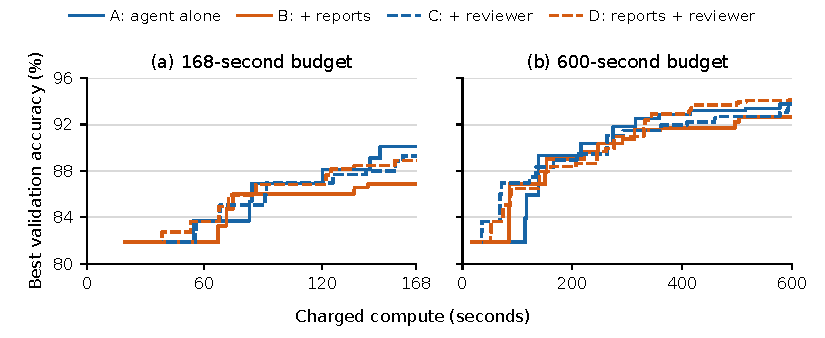
\includegraphics[width=\linewidth]{images/agent_design_curves.pdf}
\caption{Best validation accuracy versus charged compute, averaged over three seeds. The panels are separate studies with different total budgets. The curves retain the best completed candidate, so their upward steps do not imply that every experiment improved the model.}
\label{fig:curves}
\end{figure}
\FloatBarrier

\textbf{Preliminary finding.} All four designs improve substantially over the five-epoch baseline. Their ranking depends on the budget: A has the highest mean score at 168 seconds, while D leads at 600 seconds (Table~\ref{tab:results}). The larger budget was chosen after examining the first study. D leads A by 0.36 validation points and 0.28 test points at 600 seconds. Three seeds on one dataset do not establish a general winner.

\textbf{What the agents actually did.} In D's seed-2 run, longer training raised validation accuracy from 81.85\% to 87.30\%. The reviewer then recommended widening the hidden layers from [128,64] to [256,128] while keeping 25 epochs; the next experiment reached 90.40\%. Further width and duration changes reached 94.18\% validation and 94.16\% test accuracy with 454,279 parameters. The reasoning mainly follows learning curves and model capacity; this example does not establish that detailed reports caused the gains.

\textbf{Failure modes and obstacles.} After that run's best result, the reviewer recommended stopping with only 4.3 seconds left. The planner nevertheless proposed a short learning-rate probe, which hit the budget limit. In another run, B proposed 80 epochs and exceeded the 267-second per-attempt limit. Both expose weaknesses in budget planning. The random-search reference was also weakened by an interaction between class weighting and label smoothing; we therefore do not use its large gap as evidence that agents outperform conventional search.

\textbf{Next steps.} (1) Run the same A--D comparison on CIFAR-100 and the text tasks after checking feasible budgets and locking the text test-label protocol. (2) Compare how each design uses error evidence, follows reviewer advice, allocates training time, and repeats or abandons ideas; pair this analysis with additional seeds. (3) Evaluate a targeted change to budget planning or reviewer coordination, chosen from these failures, against the frozen current harness. The code can propose revised planner instructions, but recursive workflow improvement and its transfer across tasks remain untested. 

\clearpage
\begingroup
\raggedright
\renewcommand{\bibsection}{\section{References}}
\bibliographystyle{iclr2025_conference}
\bibliography{references}
\endgroup

\section{AI-Use Disclosure Statement}
ChatGPT/Codex and Claude assisted with project design, implementation, and debugging. Claude assisted with the experiment workflow and earlier result analysis. Codex assisted with the demo interface, checking saved results, and revising this report draft.

\section*{Code and Reproduction}
\coderepo\par
The project README describes dependency installation, server-side API-key configuration, running the setup chat and GPU workflow, and regenerating plots from saved results. The repository is public and can be accessed without an invitation.
\end{document}
